% README.tex
% Based on File acl2012.tex
%
% Contact: Maggie Li (cswjli@comp.polyu.edu.hk), Michael White (mwhite@ling.osu.edu)
%%
%% Based on the style files for ACL2008 by Joakim Nivre and Noah Smith
%% and that of ACL2010 by Jing-Shin Chang and Philipp Koehn


%\usepackage{setspace}
%\doublespacing

\documentclass[11pt]{article}
\usepackage{latexsym}
\usepackage{amsmath}
\usepackage{multirow}
\usepackage{url}
\usepackage{pgfplots}
\usepackage{cite}
\usepackage{framed}
\makeatother
\usepackage[hidelinks]{hyperref}
\DeclareMathOperator*{\argmax}{arg\,max}
\pgfplotsset{compat=1.14}

\begin{document}

\title{\vspace{-2.5cm}Optical Character Recognition through Convolutional Neural Networks}
\author{Jay Szeto\\ jsa143@sfu.ca \and Adrian Lim\\ aclim@sfu.ca}
\maketitle

\hrulefill

\section{Introduction}
    Optical Character Recognition (OCR) is the process of converting an image of text into computer readable text.\cite{ocr_wiki_2017} It can be used in applications such as data entry, license plate recognition, and defeating CAPTCHA anti-bot systems.\cite{ocr_wiki_2017} One approach for classification of characters involves the use of Convolutional Neural Networks (CNN).\cite{lecun_bottou_bengio_haffner_1998} This type of approach has grown more popular and complex in recent years which can be seen by the appearance of neural networks such as LeNet, ImageNet, and ResNet. \cite{lecun_bottou_bengio_haffner_1998, image_net_2012, he2016deep} Before character classification, text should be segmented into individual words or characters as incorrectly segmented text can cause improper classification. \cite{shinde_textpre-processing}
    
    In order to develop a deeper understanding of OCR using convoluted neural networks, we will be developing an OCR program that can read and classify characters in test images using the Tensorflow library. \cite{tensorflow15-whitepaper} These neural networks will be trained using font generated characters from the Char74k data set. \cite{deCampos09}
    
\section{Related Work}
    Tensorflow uses an assortment of techniques/algorithms to enable proper training.~\cite{mnist-for-ml-beginners17}. This section will focus on highlighting existing concepts and mathematical applications that are core components in the tested neural network.
    
    Tensorflow provides a step-by-step tutorial on building a LeNet style CNN with dropout for classifying the MNIST data set.\cite{tensorflow15-whitepaper, lecun_bottou_bengio_haffner_1998} This provided a good starting point for applying a CNN to the Char74k data set.

\subsection{Model Generation Function}
Tensorflow uses the softmax regression function to generate the model for assigning probabilities.  This model uses two steps:
\begin{enumerate}
  \item Collect a sum of evidence values from input belonging to a certain class/label.
  \item Convert that evidence into probabilities.
\end{enumerate}
Evidence is gathered by performing a weighted sum of the pixel intensities.  A negative weight for a pixel represents evidence that is against the image being in that class (aka label).  Positive weights are treated as evidence in favor of labeling an image to said class.

Extra evidence, called bias, were also added.  These allow the algorithm to affect the evidence with weights "more likely independent of the input".

Evidence for a class i given an input x is:
\begin{equation}
    evidence_{i} = \sum W_{i,j}x_{j} + b_{i}
\end{equation}


where $W_{i}$ is the weight and $b_{i}$ is the bias for class $i$, $j$ being an index allowing the summation of the pixels of the input image $x$.  
Once these evidences are available, a normalization of $e^x$ is required to calculate the necessary probabilities:
\begin{equation}
    softmax(evidence)_{i} = \frac{exp(evidence_{i})}{\sum exp(evidence_{j})}
\end{equation}

\iffalse
(Archived just in case)
\begin{equation}
    y = softmax(evidence)    
\end{equation}

\begin{equation}
    softmax(x) = normalise(exp(x))
\end{equation}

\begin{equation}
    softmax(x) = \frac{exp(x_{i})}{\sum_{j} exp(x_{j})}
\end{equation}
\fi

Exponentiation allows increases in evidence units to amplify our prediction probabilities, or simply the hypothesis, multiplicatively.  On the other hand, reduction in evidence amounts results in the hypothesis to reduce to a fraction of its original amount.

(The "Implementing the Regression" in first MNIST tutorial is after. However, the ItR section contains implementation details, proper placement of such info may be required...)


\subsection{Error Minimization Algorithms}
Although a method for calculating probability via evidence is available, such a model requires a training process in order to output the desired outcome.  A model's effectiveness is measured by how minimal its error margin is.  A model's loss is measured through the cross-entropy function:
\begin{equation}
    H_{y'} = - \sum y'_{i} log(y_{i})
\end{equation}
Where $y$ is the predicted probability distribution, and $y'$ is the true distribution of probabilities.  The loss function's output allows users to evaluate the amount of confidence behind a model's prediction.  

A backpropagation algorithm is used to increase prediction confidence.  By evaluating the derivative of each weight, one is able to efficiently determine the direction of improving the weights~\cite{YannLecunBottouOrrMuller98}.

Finally, a gradient descent algorithm is required to determine the appropriate direction of weight changes, and then alter weights to minimize loss.  Although TensorFlow provides a multitude of gradient descent variations, the tested neural network utilized TensorFlow's stochastic gradient descent algorithm~\cite{aGuideToLayers17}.  With all these algorithms, TensorFlow is able to use maps of weights called layers in order to process image pixel data. 


\subsection{Layers}
Neural networks consists of a different range of layer types.  Below are three different types that were used: convolutional, pooling, and fully connected layers~\cite{aGuideToLayers17}.
\begin{enumerate}
  \item \textbf{Convolutional Layer:} A layer that applies convolution filters the input image with a ReLU activation function.  Each portion of the image will produce an individual value to the output map.
  \item \textbf{Max Pooling Layer:} extracts the data from convolutional layers to reduce the dimensions of the received feature map.  Due to the max pooling algorithm, only the maximum values will persist after such downsampling.  
  \item \textbf{Fully Connected Layer:} Unlike the convolutional and pooling layers, a fully connected layer receives and outputs a map of a constant size.
\end{enumerate}


\iffalse
(Archived, since already discussed in Error Minimization Algorithms section)
subsubsection{Training}

https://www.tensorflow.org/get_started/mnist/beginners

The training of the convolutional neural network was implemented through the use of cross-entropy, backpropagation algorithm, and gradient descent optimization (caps?).
\fi


\section{Approach}

\iffalse
    - Note: ... (e.g. reader, cnn neural network layers.  one hot vectors (approach/research...?)from mnist for training, and later detecting features...)

    Note: intro to approach section here
\fi


\subsection{Pre-processing and Character Segmentation}
    
    In order to predict text from "real-life" images, the images will need to be segmented and normalized to reflect our training data. This was accomplished with a basic algorithm that first segmented the lines in the text and then segmented the characters in the text. Boxes around a test image where each line is found can be seen in figure \ref{fig:line_segmentation}. Boxes around each character found by the segmentation algorithm can be found in figure \ref{fig:character_segmentation} These characters were then re-sized and centered with a white background to normalize them with the training images.
    
    \begin{figure}
        \centering
        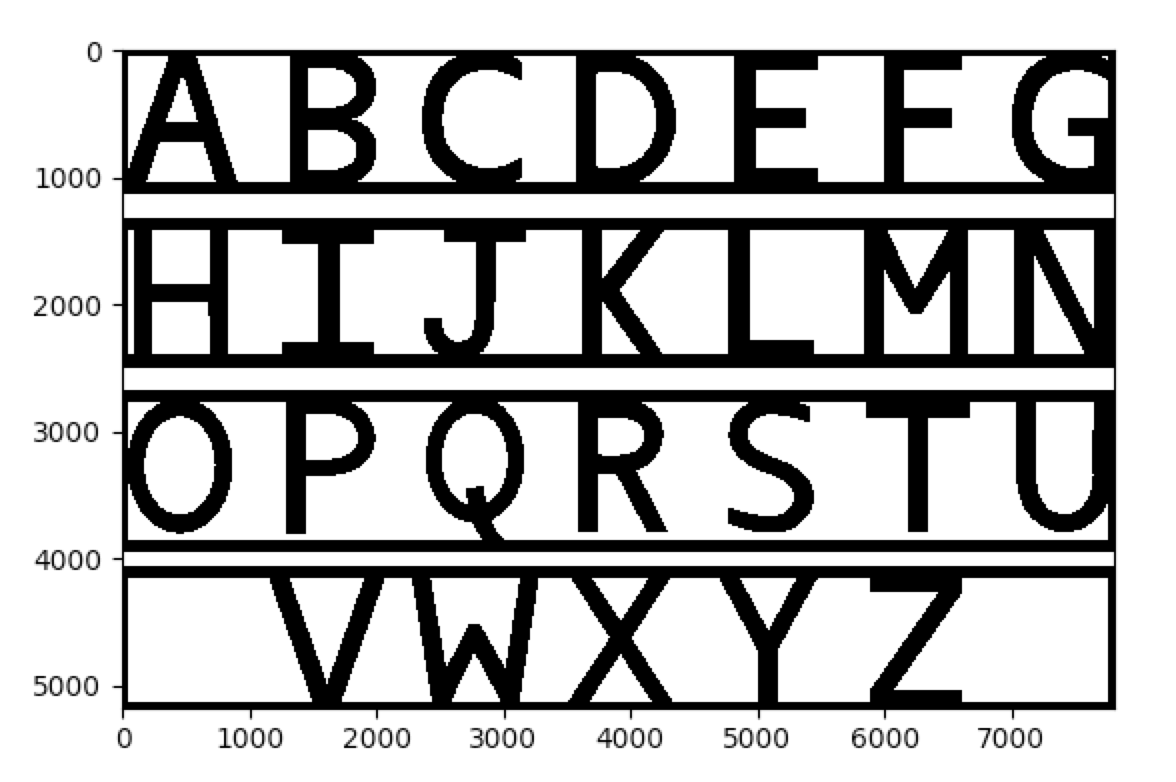
\includegraphics[scale=0.4]{line_segmentation_example.png}
        \caption{Line Detection and Segmentation}
        \label{fig:line_segmentation}
    \end{figure}
    
    \begin{figure}
        \centering
        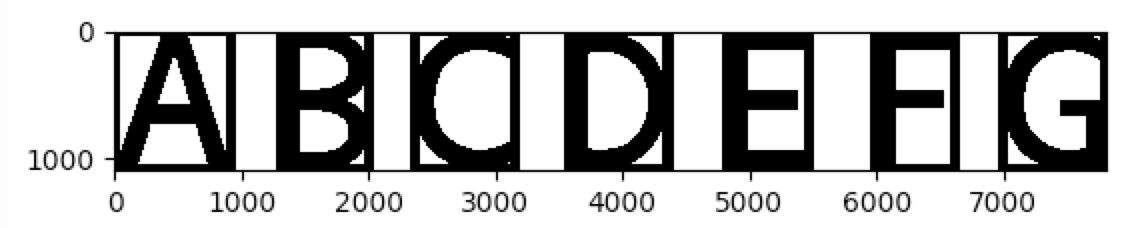
\includegraphics[scale=0.4]{character_segmentation_example.png}
        \caption{Character Detection and Segmentation}
        \label{fig:character_segmentation}
    \end{figure}

\subsection{Character Classification}

\subsubsection{The Architecture}
    To observe the effect of different parameters on the Convolutional Neural Network, we constructed multiple models.

    The first of our models was similar to the Tensorflow MNIST tutorial example except that we adjusted the final layer to output 62 different neurons as opposed to 10 to account for all of the classes of images in the Char74k data set.
    
    In our second model we added an additional convolutional layer and pooling layer and doubled the inital size of the input image.

    \begin{figure}
        \centering
        \begin{framed}
        CONV -\>> RELU -> POOL -> CONV ->RELU -> POOL -> FC -> RELU -> DROPOUT -> FC
        \end{framed}
        \caption{Model From Tensorflow Tutorial}
        \label{fig:model_1}
    \end{figure}
    
    \begin{figure}
        \centering
        \begin{framed}
        CONV -\>> RELU -> POOL -> CONV ->RELU -> POOL -> CONV ->RELU -> POOL -> FC -> RELU -> DROPOUT -> FC
        \end{framed}
        \caption{Model with additional Convolutional Layer and Pool Layer}
        \label{fig:model_2}
    \end{figure}

The Tensorflow library was used to create/structure the neural network layers~\cite{tensorflow15-whitepaper}.

\subsubsection{Predicting}

\section{Data}
The Chars74K's computer font dataset was used. This dataset contains 62992 "synthesised" characters.\cite{deCampos09}. These characters were comprised of characters of 254 different fonts with 4 different styles, normal, bold, italic, and bold and italic.\cite{deCampos09} They were chosen as the characters were centered in the middle of their images and the images were a constant size of 128 x 128. They also seemed representative of the text we were trying to recognize, text in documents.

\begin{figure}
    \centering
    
\includegraphics[scale=0.4]{training_data_sample.png}
    \caption{4 Images from the Char74k "fnt" data set}
    \label{fig:char74k_data}
\end{figure}

\section{Results}

\begin{figure}
    \centering
    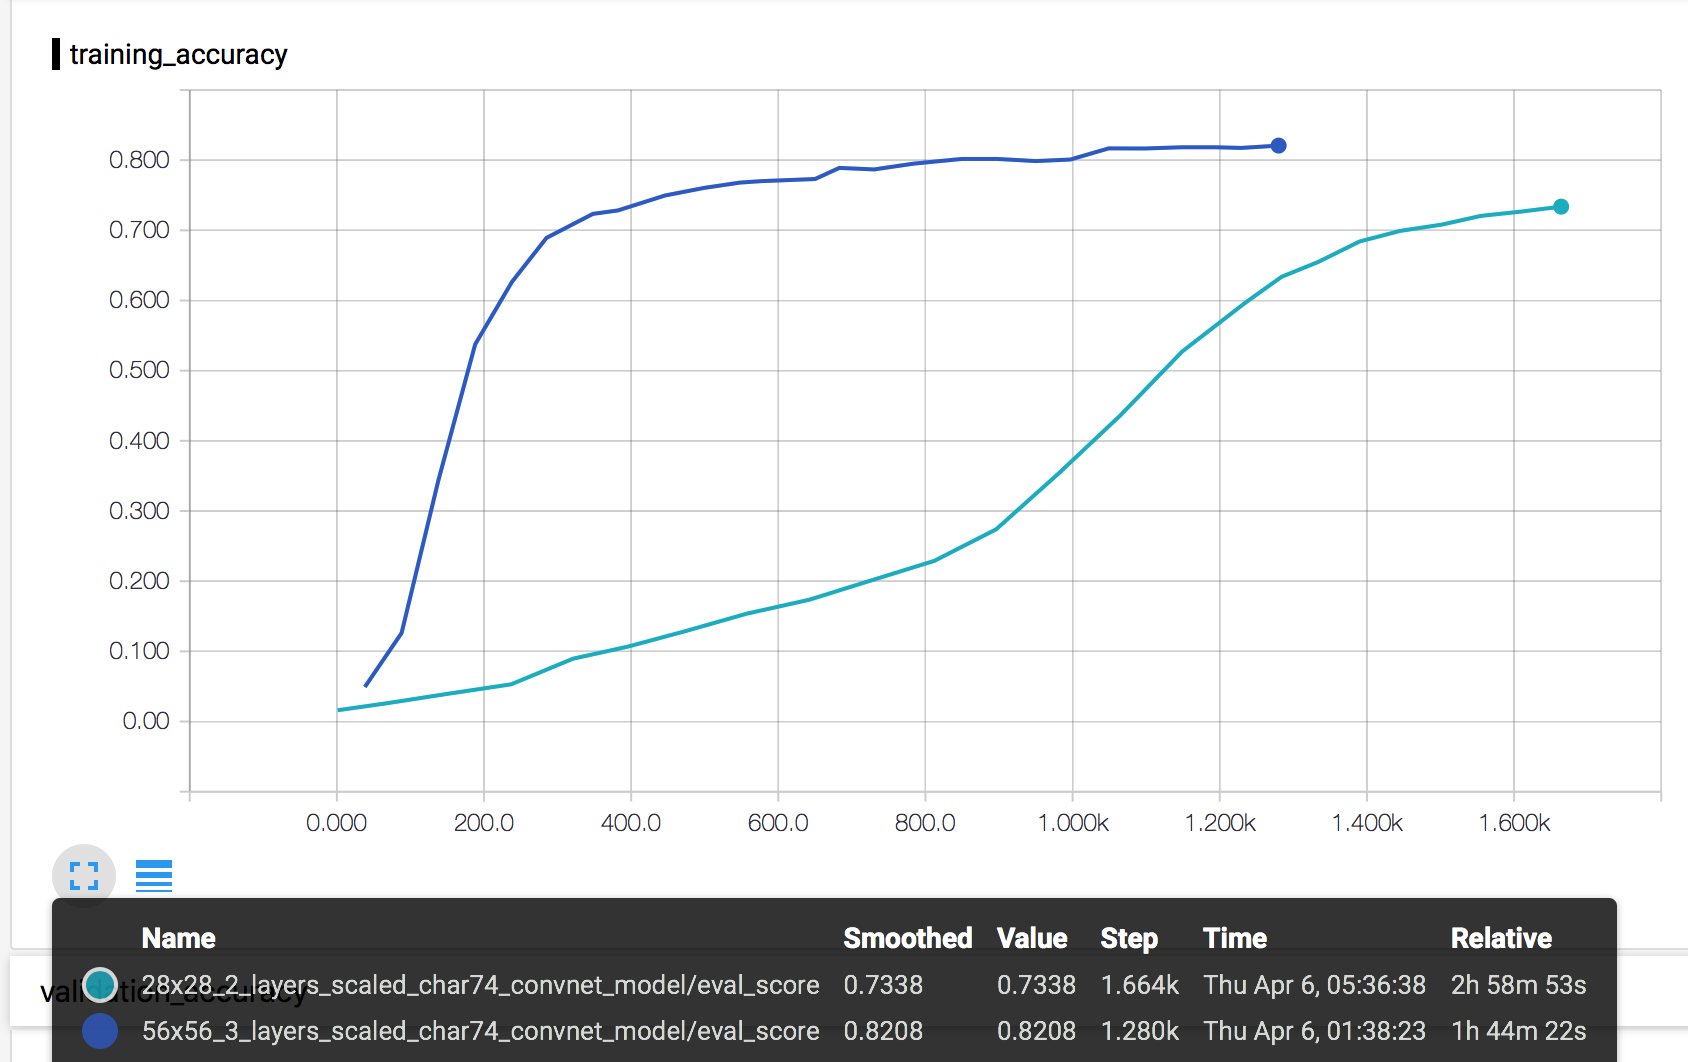
\includegraphics[scale=0.4]{training_accuracy.png}
    \caption{Training Accuracy}
    \label{fig:training_accuracy}
\end{figure}

\begin{figure}
    \centering
    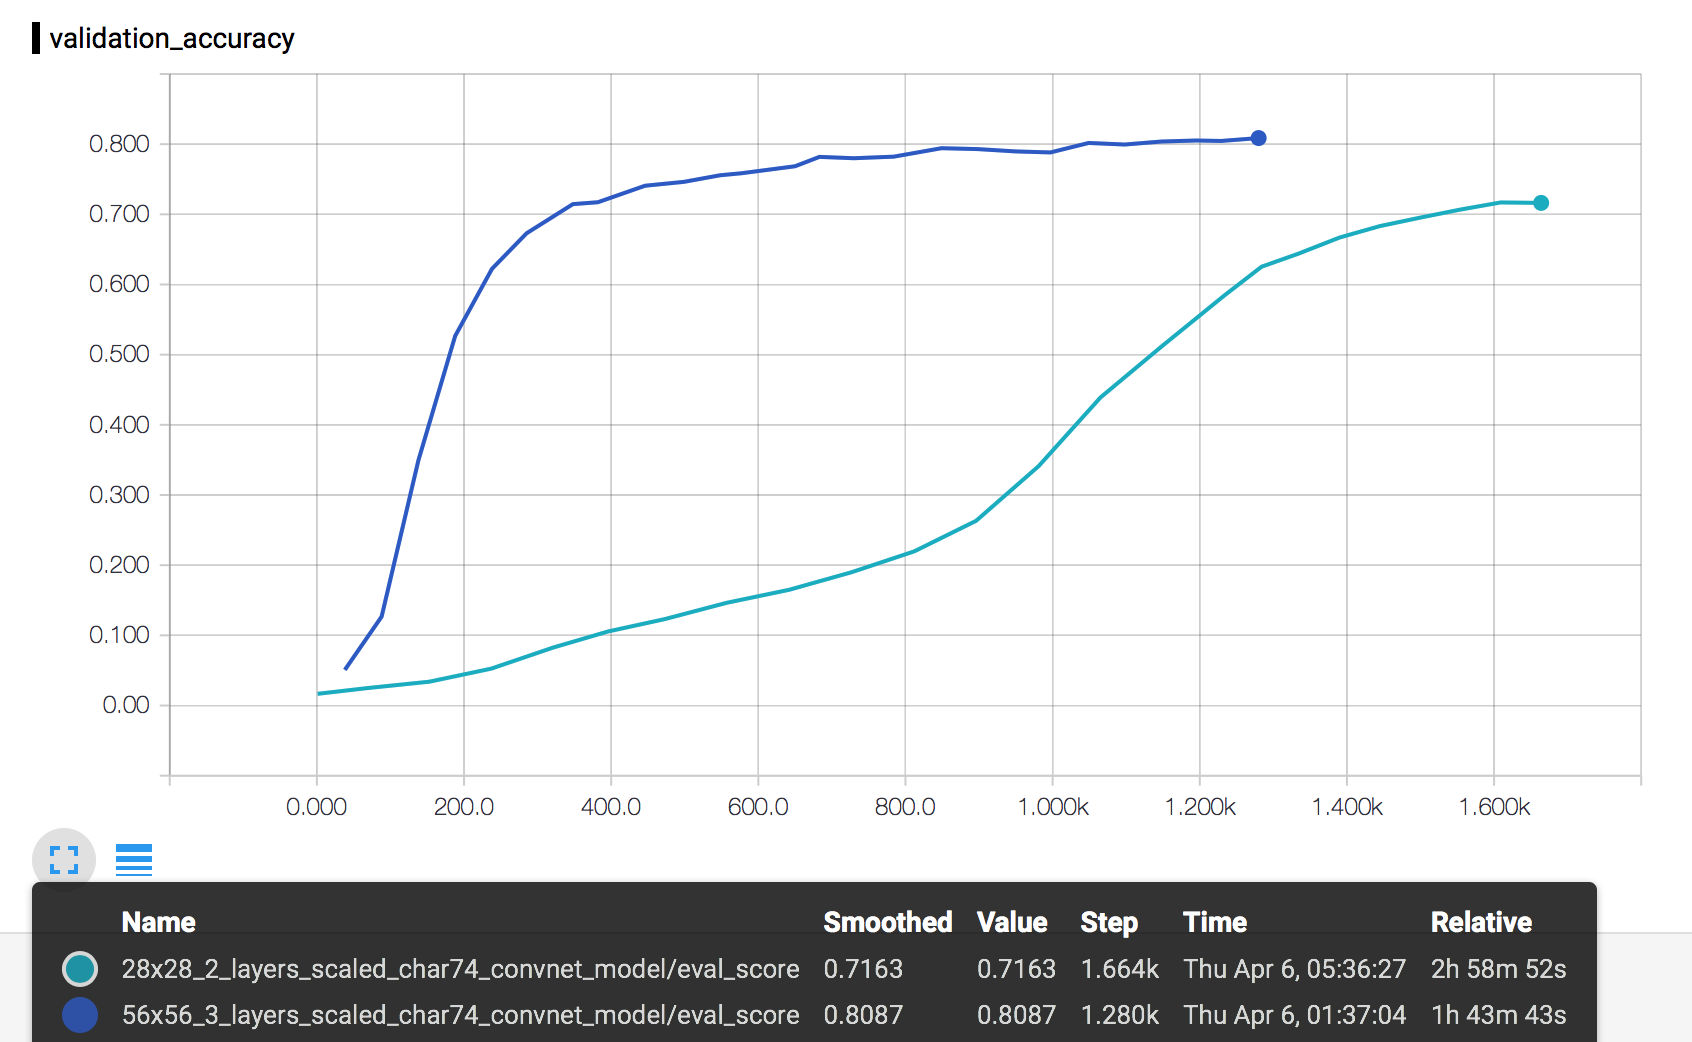
\includegraphics[scale=0.4]{validation_accuracy.png}
    \caption{Validation Accuracy}
    \label{fig:validation_accuracy}
\end{figure}

Using the Tensorflow MNIST tutorial example, we get a 74\% accuracy against our test set. A bar chart of the incorrectly predicted images can be seen in figure \ref{fig:model_1_error}

Our model with the added convolutional layer and pooling layer achieved an 81.8\% accuracy against our test set. A bar chart of the incorrectly predicted images can be seen in \ref{fig:model_2_error}.

The training set consists of 12600 images from the total char74k test set. A number of images were programatically set aside for the test set but an error caused this set to become irretrievable. For this reason 12600 random images from the complete set were chosen to replace them.

\begin{figure}
    \centering
    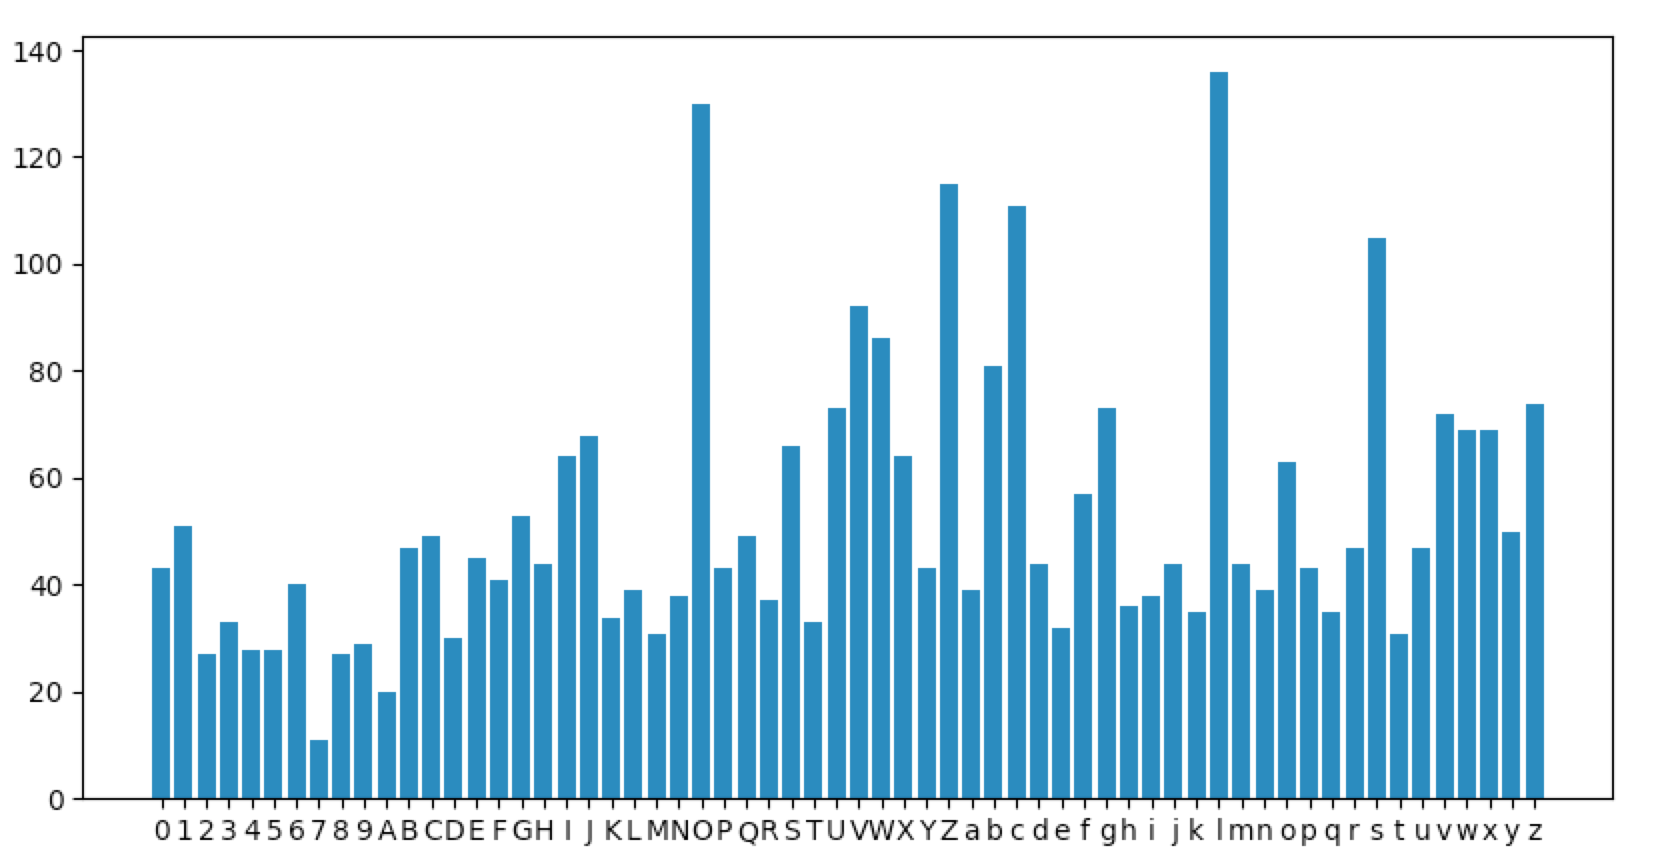
\includegraphics[scale=0.4]{model_1_errors.png}
    \caption{Bar graph showing which sample images were misclassified in the Tensorflow example prediction}
    \label{fig:model_1_error}
\end{figure}

\begin{figure}
    \centering
    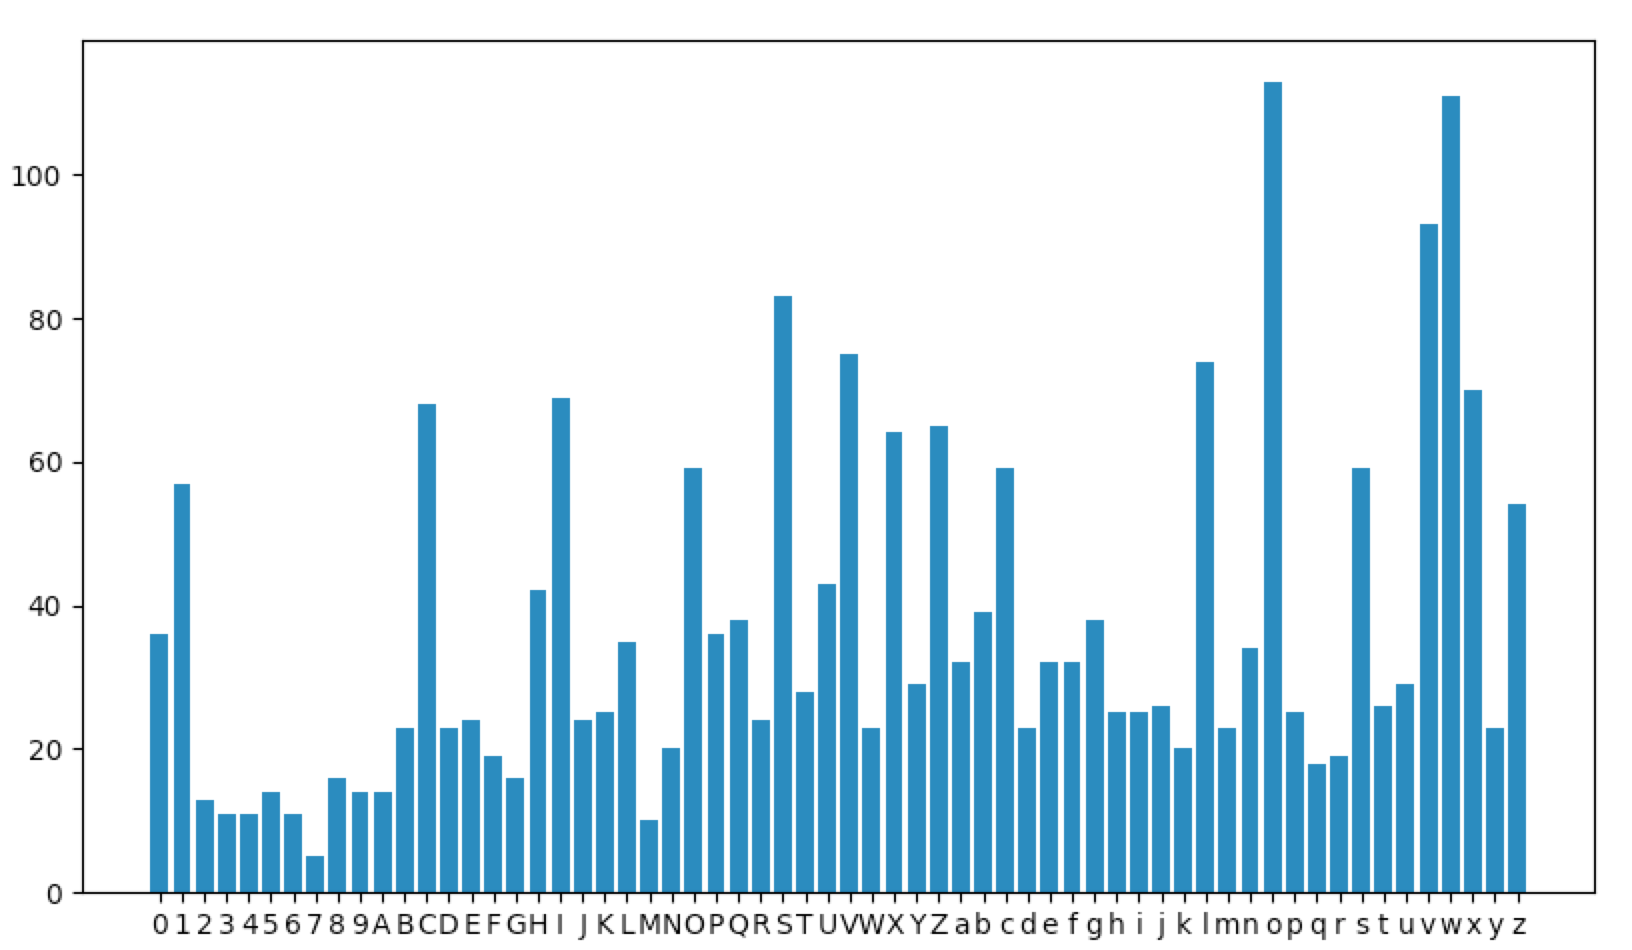
\includegraphics[scale=0.4]{model_2_errors.png}
    \caption{Bar graph showing which sample images were misclassified in the 3 convolutional and pool layer model}
    \label{fig:model_2_error}
\end{figure}

The combined character segmentation algorithm and our improved convolutional neural network was applied to a sentence taken from Wikipedia. \cite{ocr_wiki_2017} Though the neural network was not trained with symbols other than the alphabet and numbers, and the segmentation algorithm was quite basic, the output from the program was still somewhat ledge-able.

\begin{figure}
    \centering
    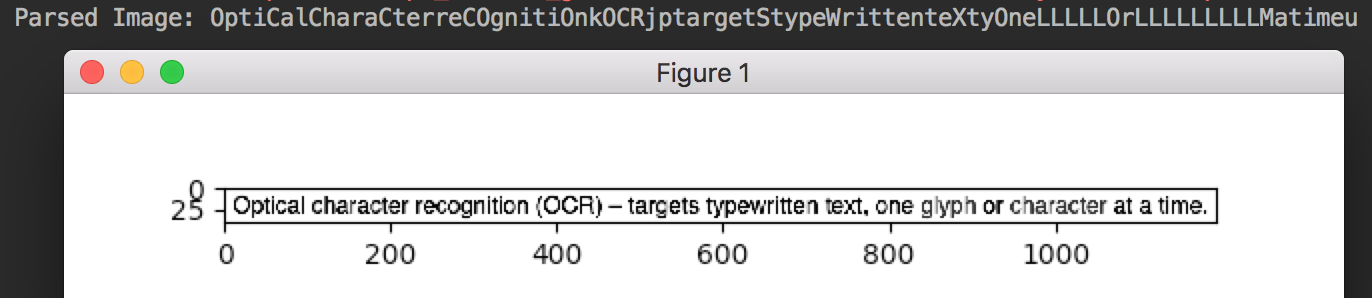
\includegraphics[scale=0.6]{sentence.png}
    \caption{OCR on a sentence taken from Wikipedia}
    \label{fig:sentence_ocr}
\end{figure}

\section{Discussion}

The results of the character segmentation shows that there is much room for improvement. However, a very basic character segmentation algorithm was written solely to apply our CNN on a more practical and interesting example.

The results show that the added convolutional layer and pooling layer in the neural network increased the accuracy of the neural network by 7.8\%. However, this may be due to over fitting as we were unable to test our network against the actual test set. We did however monitor for overfitting by plotting the accuracy in our training set and validation set which can be seen in figures \ref{fig:training_accuracy} and \ref{fig:validation_accuracy}.

Analysis of the misclassified images of the trained neural networks seems to show that the majority of errors occur in images that are extremely similar to other images, 0 and O or 1 and l, for example. Due to how the images were processed in the Char74k training set it makes sense that these images become almost indistinguishable from one another and would cause at least 1 of these characters to be misclassified more often. \ref{fig:0Oo}

\begin{figure}
    \centering
    
\includegraphics[scale=0.4]{0Oo.png}
    \caption{From left to right: 0, O, o from the Char74K training set}
    \label{fig:0Oo}
\end{figure}



\section{Future Work}
Due to the time and resource constraints, improvements to the neural network results could have been made.  Technical barriers were found when exploring the full potential of optical character recognition...



\subsection{Issues with Applying CNN Practically (how to extend further section)}
With the current resources, expanding optical character recognition to recognize words is a significant challenge.


\subsubsection{Character Segmentation}
With the given time, several variations character segmentation algorithms were considered
\begin{enumerate}
  \item Bounding Boxes per Letter
  \item Bounding Box per Textual Line (end this section by talking about noise)
\end{enumerate}

Each variation consists of its own benefits and drawbacks.  Although creating individual bounding boxes can ensure consistent padding/accuracy around letters, being able to associate letter belonging to the same line/word can become a significant challenge.  On the other hand, creating bounding boxes across lines of texts allows easier word segmentation.  However, spaces in between each word must be algorithmically measured to differentiate spaces between words.



\subsubsection{Text Extraction from Images}
Similar to license plate detection, an attempts to extract text from an internet meme image indicate that a sophisticated algorithm is required to accurately extract images.
A quick algorithm might involve applying filters to emphasize white text, causing high intensity pixels to be extracted from an image.  However, the algorithm does not yield accurate results in all cases, since noise with similar intensities will also be extracted.


\section{Conclusion}
...Final message/summary of key points here?


\iffalse
Option: talk about Matt's ramblings on "Number plate recognition with Tensorflow" algorithm
and compare it to ours. (His approach, more training images/test data that are also indepth)
sliding window implementation to locate text region.
- pros: can detect meme text better
- cons: dataset for training images of text on pictures (meme format) not available
    - his algorithm only shows him detecting one plate (or line of text in the case of memes)
    - datasets are extensive example had ~3 GB of background images) tar file 36 GB
        - extracting tar file gets 108,634 images \url = {https://github.com/matthewearl/deep-anpr/blob/master/README.md}
    - his approach uses a specific font (good if meme follows consistent font, which isn't always the case since meme's are not regulated)


-------------------
Below are some brainstormed ideas for future work (Not exhaustive.  Section open to other ideas): 

- what can be improved 
    - e.g. character segmentation, 
    - ways to deal with noise, 
    - increasing number of layers...
    - etc
    
- what could we have done (if we had more time or resources...
    - e.g. specific details of how to char segmentation
    - noise dealing details
    - using specialized training images for specific
        reading situations
    
- how can we extend this further? What challenges will one might have to face?
    - e.g. algorithm to read documents...
    - text on meme reader
    - text on textbook reader (digital source)
    - text on a piece of paper (can easier be more noise)
        - but as similar in accuracy when reading from digital source, (suppose we read from high definition image of real textbook page to convert into digital source?
            - more issues if we make such a product since currently we assume text is parallel/horizontal
\fi

\iffalse
*Note: Future improvement, research showed that performing OCR (using...) is more effective in analyzing characters at the word level
http://yann.lecun.com/exdb/publis/pdf/lecun-95b.pdf

*Note: lowercase letters same "size" as uppercase in dataset
http://yann.lecun.com/exdb/publis/pdf/lecun-01a.pdf



\section{Note to Self/Sources/References?(use bibliography instead of this section)}
Certain Tutorials were provided by Tensorflow regarding how to create our own MNIST Convolutional Neural Networks
\begin{verbatim}
https://www.tensorflow.org/get_started/mnist/mechanics
https://www.tensorflow.org/tutorials/layers
\end{verbatim}

\fi



\clearpage
\bibliography{project}
\bibliographystyle{ieeetr}

\end{document}
